\chapter{Simulazione}
Data la straordinarietà degli eventi che erano in corso dal punto di vista sanitario nel nostro paese si è reso necessario svolgere gran parte del lavoro in modalità a distanza e quindi senza la possibilità di testare il modello matematico appena ottenuto e i successivi risultati dovuti all'azione di controllo sul V.A.B. Il lavoro quindi è stato svolto per la maggior parte sfruttando il tool \textit{Simulink} di Matlab che è, in poche parole, un risolutore di equazioni differenziali.

Abbiamo così adottato una metodologia di lavoro basata su prototipi sempre più simili a quello che dovrebbe essere il sistema reale.
\section{Simulazione del sistema reale}
Il primo compito che abbiamo risolto è stato quello di implementare le equazioni differenziali ottenute nel capitolo precedente:
\begin{itemize}
	\item $\ddot{\phi} = f_{\ddot{\phi}} (M_c,\theta,\dot{\theta},C_m)$
	\item $\ddot{\theta} = f_{\ddot{\theta}} (M_c,\theta,\dot{\theta},C_m)$
\end{itemize}

Dove $M_c$ sarebbe la massa del passeggero, $\theta e \dot{\theta}$ lo stato del sistema e $C_m$  la coppia erogata dal motore. Si può notare come entrambe le equazioni differenziali siano indipendenti dalla coordinata libera $\phi$.
 \begin{figure}[H]
	\centering   	
	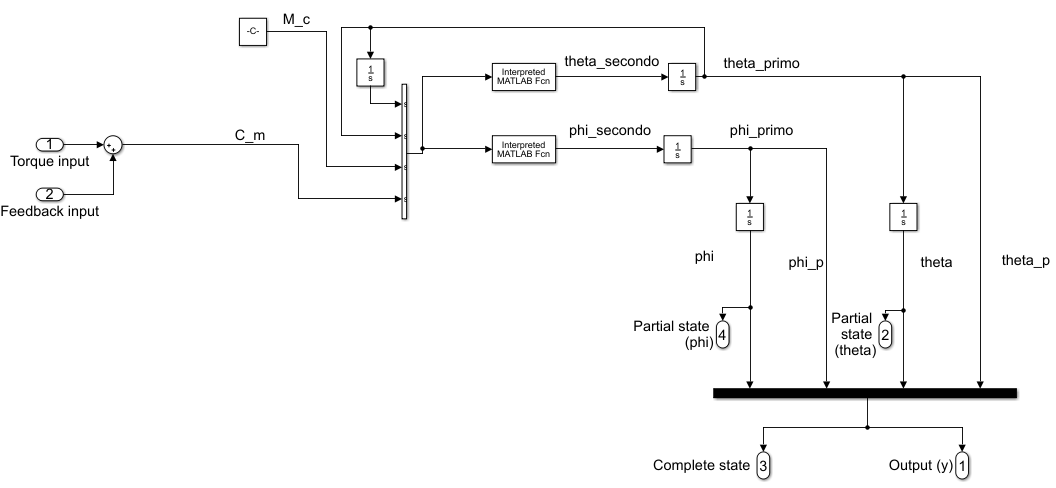
\includegraphics[width=1\textwidth]{Immagini/non_linear_system.png}
	\caption{Implementazione simulink delle equazioni differenziali}
	\label{fig:non_linear_system}
\end{figure}
In Fig.\ref{fig:non_linear_system} le \textit{interpreted function} altro non sono che  $f_{\ddot{\phi}}$ e $f_{\ddot{\theta}}$. A valle di esse sono presenti degli integratori che permettono di ottenere lo stato $x$ completo del sistema. Si può facilmente notare come $\dot{\theta} e \theta$ siano collegate direttamente all'input delle \textit{interpreted function}.
Si è dunque proceduto a  simulare il sistema per verificare la bontà di quanto ottenuto; in particolare, il sistema in anello aperto, dovrebbe oscillare all'infinito vista la mancanza di attriti nel modello.
\\
TODO grafico e foto sistema simulink non lineare anello aperto e chiuso
\\
Si è inoltre creato un altro modello sfruttando il sistema lineare ottenuto prima  con l'obbiettivo di semplificare il problema e di velocizzare le simulazioni con lo scopo di testare rapidamente nuove tecniche di controllo che se avessero dato esito positivo sul modello lineare sarebbero poi state testate sul simulink che imita il comportamento reale del sistema.
\begin{figure}[h]
	\centering   	
	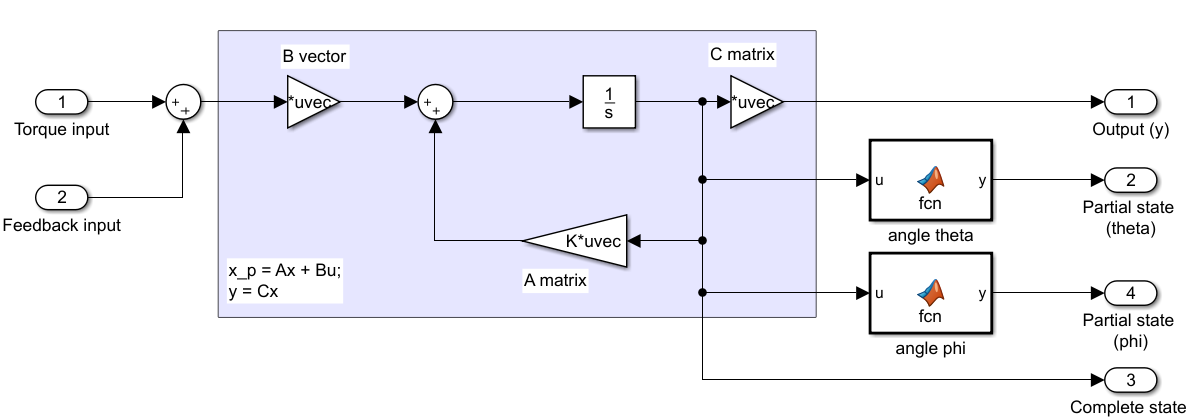
\includegraphics[width=1\textwidth]{Immagini/linear_system.png}
	\caption{Implementazione simulink del sistema linearizzato}
	\label{fig:linear_system}
\end{figure}

TODO grafico e foto sistema lineare anello aperto e chiuso
\\
In questo caso, la simulazione in anello aperto mostra che il sistema diverge; questo perché la linearizzazione ha senso attorno al punto di equilibrio da cui è stata ottenuta, distante da quel punto il sistema lineare non approssima più il sistema reale ed anche un eventuale controllo ottenuto da esso non garantisce buone performance distante da quel punto.\\
TODO aggiungere immagini posizionamento poli per dimostrare instabilità\\
\section{Controllore}
Il problema della scelta del controllore è stato risolto mediante l'utilizzo dell'assegnazione degli autovalori ottenuti tramite retroazione dello stato; si affronta quindi un problema di regolazione: il moto del sistema è composto completamente dal moto libero che si vuole controllare e annullare in un tempo a piacere. Il posizionamento dei poli, e quindi la scelta del guadagno del regolatore, va eseguita sul solo sistema lineare:
\begin{figure}[h]
	\centering   	
	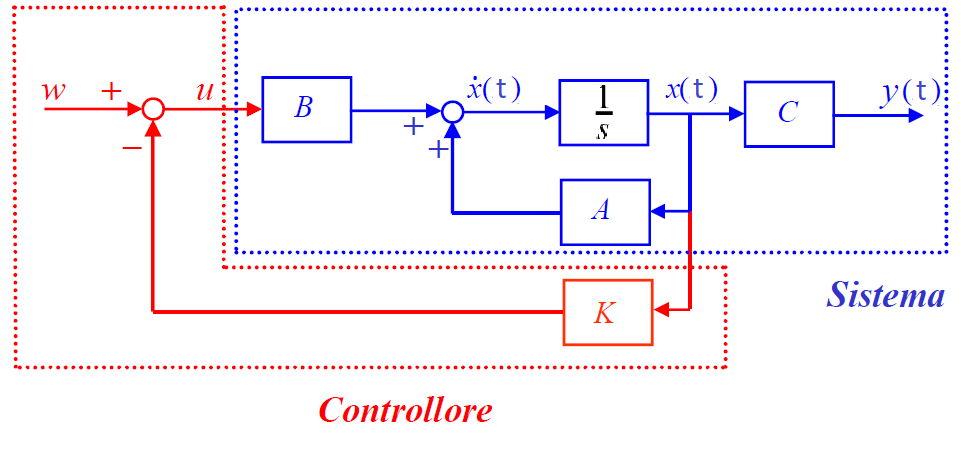
\includegraphics[width=0.70\textwidth]{Immagini/feedback_state.png}
	\caption{Schema concettuale del controllo,\cite{feedback_state}}
	\label{fig:feedback_state}
\end{figure}
Gli steps necessari per il posizionamento dei poli sono i seguenti:
\begin{itemize}
	\item 
	contenuto...
\end{itemize}
